\chapter{Hello World}
Python is a programming language, developed by the Python Software Foundation and released under the PSFL License. I quote Wikipedia: \begin{quotation}
`Python is an interpreted, high-level, general-purpose programming language. Created by Guido van Rossum and first released in 1991, Python's design philosophy emphasizes code readability with its notable use of significant whitespace. Its language constructs and object-oriented approach aim to help programmers write clear, logical code for small and large-scale projects.
\end{quotation}
For those who have never programmed in their lives, Python offers an easy in of sorts, as the language is very easy to both read and use.
\section{Python installed?}
To check if you have Python already installed, open the command prompt and type \begin{quote}
Python
\end{quote}
If Python is installed, the command prompt should reply
\begin{quote}
Python 3.8.3 (tags/v3.8.3:6f8c832, May 13 2020, 22:37:02) [MSC v.1924 64 bit (AMD64)] on win32\\
Type "help", "copyright", "credits" or "license" for more information.\\
$>>>$
\end{quote}
However, if you don't see a message like above, but instead see:
\begin{quote}
'python' is not recognized as an internal or external command,\\
operable program or batch file.
\end{quote}
then, you don't have a copy of Python on your computer.
To install Python, go to www.python.org/downloads/ and follow the instructions\\
Now that all of us have Python installed on our computrs, we may begin or exploration of the language.
\section{First program}
Finally, our first program. Our aim is to print the statement "Hello World" (Interestingly, the tradition began with Ritchie \& Kerningham's book `The C Programming Language')\begin{quote}
print("Hello World!")
\end{quote}
Would simply return:
\begin{quote}
Hello World!
\end{quote}
In Python 3, the statement \emph{print()} was used to print a statement, which in the above case was a string which was enclosed in "double quotes". 
\section{More Printing}
If we so desire, we may also print multiple strings at the same time using the \emph{print()} function as shown:
\begin{quote}
print("Hello World!","Hoorah!!")
\end{quote}
which would return
\begin{quote}
Hello World! Hoorah!!
\end{quote}
The \emph{print()} function inserts a newline after printing the arguments passed to it. So in other words,
\begin{quote}
print("Hello World!","Hoorah!!")
\end{quote}
and 
\begin{quote}
print("Hello World!")\\
print("Hoorah!!")
\end{quote}
Would return two different outputs as shown
\begin{quote}
Hello World! Hoorah!!
\end{quote}
and 
\begin{quote}
Hello World!\\
Hoorah!!
\end{quote}
respectively.\\
To force the printing of a newline, we use "\textbackslash n" in our string as shown.
\begin{quote}
print("Hello World! \textbackslash n Hoorah!!")
\end{quote}
The above script returns the same output as:
\begin{quote}
print("Hello World!")\\
print("Hoorah!!")
\end{quote}
But the former is generally preferred for the sake of brevity.
\section{Variable Variables}
Now that we have started using the \emph{print()} function, we may further explore it.\\
the print function can also print the value of variables.
\begin{quote}
somevariable="Hello World, I am a variable"\\
print(somevariable)
\end{quote}
returns
\begin{quote}
Hello World, I am a variable
\end{quote}
The variable can the be reset to another value if needed.\\ In short, a single 'equals' mark indicates assignment of a variable.
The entire process can be described as: 
\begin{figure}[h]
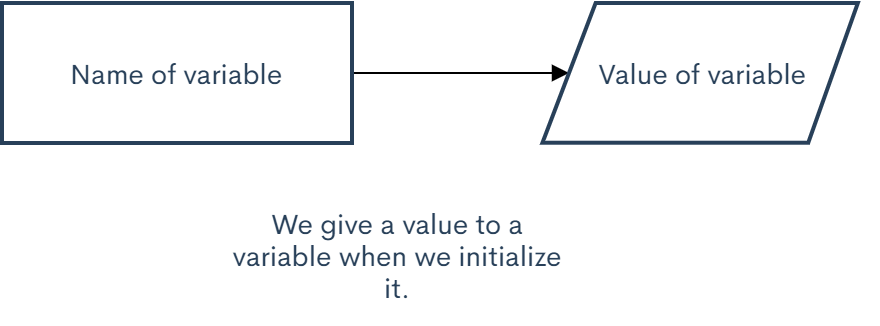
\includegraphics[scale=0.25, right]{variableflowchart}
\end{figure}
\\
Every variable, can be initia;ized both implictly and explicitly. In both cases, a value is assigned to it. If it is explicitly defined, then we use a single `equal' to sign (=)
\section{Arithmetic}
Python, like most programming languages has basic math in it's Standard Library. The four symbols, `+' `-' `*' and `/' are used with both variables an constants.
\newpage For example to find and print the product of 256 and 456, we can use:
\begin{quote}
a=256\\b=456\\c=a*b\\print(c)
\end{quote}
or
\begin{quote}
a=256\\b=456\\print(a*b)
\end{quote}
or
\begin{quote}
print(256*456)
\end{quote}
While all three of them return the same result, all three of them have diiferent uses. The first is used while `Debugging', the second in most programs where brevity is needed and the third while using Python as a calculator.\\
The  \emph{print()} function takes both variables and strings as inputs and can concatenate the values of both inplace. thus, to give more clarity to the end user, a statement may also be included. for example, to calculate the value of 234*235 and give a statement about the same, the following two scripts may be used
\begin{quote}
a=256\\b=456\\print("The product of the given variables is" ,  a*b)
\end{quote}
or
\begin{quote}
a=256\\b=456\\c="The product of the given variables is"  \\print(c,a*b)
\end{quote}
Multiple such variables may be referred so, a similiar but better program can also list the values that are being multiplied by name, ie.  
\begin{quote}
a=256\\b=456\\print("The product of " , a ,",", b ,"is" ,  a*b)
\end{quote}
\section{Excercise}
\begin{enumerate}
\item Write a program to convert \emph{Celsius} to\emph{Fahrenhiet} for a given temperature $t=45^{\circ}$C.
\item Write a program that calculates the average of three numbers $189086,127809,1567801$.
\end{enumerate}

